\begin{figure}
	\centering
	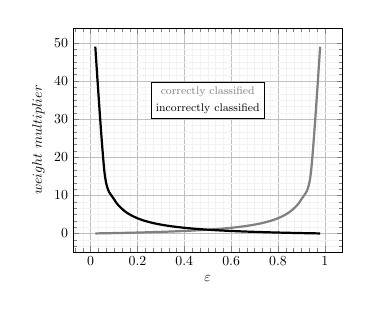
\begin{tikzpicture}[
		scale=0.5
	]

		\begin{axis}[
			domain=0.02:0.98,
			minor tick num=5,
			grid=both,
    			grid style={line width=.1pt, draw=gray!10},
    			major grid style={line width=.2pt,draw=gray!50},
			legend pos=outer north east,
			xlabel={$\varepsilon$},
			ylabel={$weight\ multiplier$}
		]
    			\addplot[no marks,ultra thick,smooth,gray]{exp(-(ln((1-x)/x)))};
			\addplot[no marks,ultra thick,smooth,black]{exp(ln((1-x)/x))};

			\node[align=center,fill=white,draw=black] at (axis cs:0.5,35) {\textcolor{gray}{
				\footnotesize{correctly classified}}\\ \footnotesize{incorrectly classified}
			};
    		\end{axis}
		
	\end{tikzpicture}
\end{figure}